%\documentclass{uai2023} % for initial submission
% \documentclass[accepted]{uai2023} % after acceptance, for a revised
% version; also before submission to
% see how the non-anonymous paper
% would look like
%% There is a class option to choose the math font
%\documentclass[mathfont=ptmx]{uai2023} % ptmx math instead of Computer
% Modern (has noticable issues)
\documentclass[mathfont=newtx]{uai2023} % newtx fonts (improves upon
% ptmx; less tested, no support)
% NOTE: Only keep *one* line above as appropriate, as it will be replaced
%       automatically for papers to be published. Do not make any other
%       change above this note for an accepted version.

\usepackage{graphicx}

%s\usepackage{amsmath,amssymb} % define this before the line numbering.




%% Choose your variant of English; be consistent
\usepackage[american]{babel}


%% Some suggested packages, as needed:
\usepackage{natbib} % has a nice set of citation styles and commands

\renewcommand{\bibsection}{\subsubsection*{References}}
%\usepackage{mathtools} % amsmath with fixes and additions
% \usepackage{siunitx} % for proper typesetting of numbers and units


%for table
\usepackage{booktabs}
%subfigure


\usepackage{svg}
\usepackage{float}
\usepackage{balance}
\usepackage{caption,subcaption}

\newcommand{\MethodnameLong}{Federated Learning for distribution skewed data using sample weights: FedDisk}
\newcommand{\MethodnameShort}{FedDisk}

\newcommand{\px}[2]{p_{#1}(\mathbf{x_{#2}})}
\newcommand{\qx}[2]{q_{#1}(\mathbf{x_{#2}})}

\newcommand{\Prob}{\mathcal{P} }
\newcommand{\prob}{\mathcal{P} }

\newcommand{\x}{\mathbf{x}}
\newcommand{\ubold}{\mathbf{u}}

\newcommand\parties{100}

%%%%%% for privacy section
\usepackage{stmaryrd}

%%%%%%%% for saving spaces
\usepackage[subtle]{savetrees}
\setlength\abovedisplayskip{0pt}
\setlength\belowdisplayskip{0pt}

\titlespacing\section{0pt}{12pt plus 4pt minus 2pt}{0pt plus 2pt minus 2pt}
\titlespacing\subsection{0pt}{12pt plus 4pt minus 2pt}{0pt plus 2pt minus 2pt}
\titlespacing\subsubsection{0pt}{12pt plus 4pt minus 2pt}{0pt plus 2pt minus 2pt}


%%%% End saving spaces

\title{\MethodnameLong}
% The standard author block has changed for UAI 2023 to provide
% more space for long author lists and allow for complex affiliations
%
% All author information is authomatically removed by the class for the
% anonymous submission version of your paper, so you can already add your
% information below.
%
% Add authors
\author[1]{Hung Nguyen}
\author[2]{Morris Chang}
\author[3]{Peiyuan Wu}
% Add affiliations after the authors
\affil[1]{%
	Electrical Engineering Dept.\\
	University Of South Florida\\
	Tampa, Florida , USA\\
	nsh@usf.edu
}
\affil[2]{%
	Electrical Engineering Dept.\\
	University Of South Florida\\
	Tampa, Florida , USA\\
	chang5@usf.edu
}
\affil[3]{%
	Electrical Engineering Dept.\\
	National Taiwan University\\
	Taiwan\\
	peiyuanwu@ntu.edu.tw
}



\begin{document}
	
	\maketitle
	
%%%%%%%%% ABSTRACT
\begin{abstract}
   One of the most challenging issues in federated learning is the non-IID data issue. In a federated learning setting, it is expected that clients contribute the same type of data but might collect it in different ways from different resources. Thus, the data distributions might be different. This work focuses on improving federated learning performance for skewed data distribution across clients. We start from the fundamental concept of empirical risk minimization and theoretically derive a solution for adjusting the distribution skewness using sample weights. To determine sample weights, we implicitly exchange density information by leveraging a neural network-based density estimation model, MADE. We then can adjust clients' data distribution without exposing their raw data. Our experiment results on three real-world datasets show that the proposed method not only improves federated learning accuracy but also significantly reduces communication costs compared to the other experimental methods. 
\end{abstract}

%%%%%%%%% BODY TEXT
\section{Introduction}
Since the demand for massive data in artificial intelligent machines, the concept of federated learning (FL) was first introduced in 2017 \cite{OriginFL}, which is a collaboratively decentralized learning framework. In contrast to centralized learning approaches (in which datasets are sent to an aggregator), FL encourages data holders to contribute without the privacy concern of exposing their raw data. For example, several hospitals holding patient records would participate in a machine learning system to provide better disease predictions via a FL framework without the concern of privacy disclosure. Since then, FL has been seen in various applications in different fields \cite{abs-1811-03604,yadav_federated_2022,feki_federated_2021,zhai_dynamic_2021}. 

%FL can be categorized into two schemes: cross-silo and cross-device. Cross-device is a setting that is more concerned about participating thousands of devices (e.g., personal phones, sensors, wearable devices), such as an IoT system. Cross-silo is more concerned about the setting that enables FL to learn from a number of databases, and each of them contains a significant trunk of data. In this study, we focus on this cross-silo category. 

To learn a model utilizing data from multiple clients without directly accessing to clients' data, authors in \cite{OriginFL} introduced Federated Averaging (FedAvg) and demonstrated its robustness. The main idea is that clients (data holders) involve in a model training process by exchanging local models' weights instead of exchanging raw data. One of the main concerns in FL is that the data might come from different sources and have different distributions. Thus, FL performance is significantly reduced because this violates a fundamental machine learning assumption that data should be independent and identically distributed (IID). The FL over non-IID data has been shown in existing works \cite{ZHU2021371,Sahu2018OnTC,9392310,abs_1905_06641,Shen2020FederatedML,9155494,abs-2102-02079,abs-2005-11418} that its performance deteriorates dramatically. In this work, we focus on tackling the non-IID data issue in a federated learning system, in which the collected data feature distribution is skewed. The skewness might be caused by many different reasons. For example, clients might perform different sampling methods, apply different normalization methods, or sample using different devices. 

Over the past few years, there have been a number of approaches aiming at reducing non-IID data impacts. While many current works focus on the skewed label distribution, there are only limited approaches considering skewed feature distribution data which is very common in various fields, e.g., medical images collected from different x-ray machines. Authors in \cite{Zhao2018FederatedLW} explained the performance reduction as the problem of weight divergence. They then proposed an alleviation by combining local data with global shared data to train each client. However, it raises the concern of privacy violation with the shared data. Li et al. illustrated in their work (FedBN) \cite{li2021fedbn} that Local Batch Normalization would help to reduce the problem of non-IID data. FedBN suggests clients to not synchronize local batch normalization parameters with the global model. Sahu et al. introduce FedProx \cite{FedProx} to solve the weight-divergence issue by proposing a loss function which constrains the local models to stay close to the global model. FedDNA \cite{fedDNA} shares statistical parameters of models (means and variances) and aims at finding averaging weights for each client's model to minimize models' weights divergence across clients. However, as this only considers the aggregating weights for each model, the improvement is minor. FedNova \cite{fednova} suggests to normalize local weights before synchronizing with the aggregator. FedMA \cite{fedma}, AFL \cite{AFL} and PFNM \cite{pfnm} consider combinations of layer-wise parameters and provide an aggregation of such parameters to alleviate the non-IID issue. In FedRod \cite{FedRod}, Chen and Chao deal with the non-IID issue by learning hyper-networks locally which results in personalized classifiers for clients and clients' class distributions. Recently, Tan et al. \cite{FedProto} tackle the non-IID data issue by exchanging representation vectors of samples in a given class instead of model's parameters, enable clients to have personalized model architecture. However, these suggestions do not directly consider the data distribution skewness at the data level, which could lead to performance reduction and convergence slowth.    

Different from centralized learning frameworks, the non-IID issue is challenging in FL because of the limited access to client's raw data. To overcome this, we propose an algorithm that implicitly leverages statistical information of client data to alleviate the distribution skewness impact. Our method only requires clients to exchange additional model weights using a typical FL procedure. The proposed method aims to exchange statistical information to generate sample weights to adjust distribution skewness at the sample level. After acquiring the adjusting weights, the machine learning model can be trained under a typical FL framework. Similar to a typical FL framework, the proposed method does not require clients to expose their private data.
Our contributions are as follows:
\begin{enumerate}
\item Provide a theoretical base to deal with skewed feature distribution data for federated learning by adjusting sample weights derived from the machine learning empirical risk.  
\item Provide a practical solution to mitigate the problem of learning from non-IID data for the FL framework without sharing clients' draw data. It not only helps to improve the classification accuracy of the global model but also accelerates the model convergence process, thus minimizing communication costs.
\item Several experiments were conducted on three datasets, including MNIST, non-IID benchmark dataset FEMNIST and real-world dataset Chest-Xray. The results demonstrate that the proposed method outperforms other experimental methods in classification accuracy and dramatically reduces the communication cost.
\item As the proposed method needs to exchange additional information, we also provide a theoretical analysis to analyze the potential privacy leakage. We showed that the leakage information becomes insignificant when the number of clients increases. 
\item To our best knowledge, the proposed method is the first method utilizing data distribution information and sample weights to tackle the FL Non-IID issue.   
\end{enumerate}

%The rest of this paper is organized as follows. Section \ref{sec:problem} introduces our problem in a scenario where clients hold different distribution datasets. Section \ref{sec:made} introduces a neural network-based model is leveraged in our work to carry density information. Our proposed solution is introduced in Section \ref{sec:methodology}. We provide a privacy leakage analysis in Section \ref{sec:privacyAnalysis} as the proposed method indirectly exchanges distribution information. Section \ref{sec:experiments} shows our experimental results and illustrates the proposed method's performance. Section \ref{sec:conclusion} summarizes our study and discusses the future work to improve the proposed method.        
\section{Scenario}
\label{sec:problem}
In this section, we introduce and formulate the scenario of FL with skewed feature distribution across clients. 
Our scenario is a learning collaboration between $K$ clients to build a global classification model that maximizes the global accuracy given arbitrary data. Each client holds a number of individual records that they are not willing to share with others due to privacy concerns. This study focus on preventing the performance of the global model from deteriorating because of the distribution skewness issue \cite{survey} across clients.

We denote the data and associated labels held by client $k$ $\in$ $\{1,...,K\}$ as $ \{( \mathbf{x}_k^i,y_k^i )\}_{i=1}^{N_k}$ where $ \mathbf{x}_k^i \in \mathbb{R}^d$ and $y_k^i \in \mathbb{N}$. Instead of learning each model for every client $f(\mathbf{w}_k)$ (where $f(\cdot)$ demotes local inference models and $\mathbf{w}_k$ is the model's parameter of the $k^{th}$ client), the objective is to maximize the performance of a global model $g(\mathbf{w})$ ($g(\cdot)$ approximates the global inference model and $\mathbf{w}$ is the global model's parameter) that is resilient to data skewness.  

\section{Preliminary: Masked Autoencoder for Distribution Estimation (MADE) }
\label{sec:made}
The proposed method asks the clients to share additional model weights that carry their local datasets' distribution information instead of sharing the raw data. We utilize a neural network-based density estimation, namely, Masked Autoencoder for Distribution Estimation (MADE) \cite{MADE}. This section briefly introduces MADE.

MADE is designed to estimate the probability distribution of input components (e.g., pixels in an image). MADE assumes input components are dependent instead of independent, which is relevant in many applications. For example, MADE can decompose the distribution of an instance $\textbf{x}$ consisting d components $x_1, x_2, x_3, ..., x_n$ as follows:
\begin{equation}
	\label{eq:MADE_decomposition}
   p(\mathbf{x}) =   p(x_1|x_2,x_3,..,x_n) \cdot p(x_2|x_3,...,x_n) 
					...p(x_{n-1}|x_n) \cdot p(x_n). 
\end{equation}
 
For implementation, MADE poses the constraint on a neural network model that each output component in a certain layer only connects to its dependent input components in the previous layer. Masks are created based on such principle, and applied to the weights of the model.
%Specifically, MADE assigns each unit in a hidden layer an integer $\textit{m}$ between $1$ and $D-1$, where $D$ is the number of dimensions. Denote $\textit{m(k) } $ as the maximum number of units in the previous layer to which the $\textit{k}^{th}$ hidden unit can connect, the weight mask $M$ is then formulated as follows:
%$
% M_{k,d} = 1_{m(k) \geq d} = 
%				 \begin{cases}
%				  1 & \text{if \textit{m(k)} $\geq$ d }\\
%				  0 & \text{otherwise,}
%				 \end{cases} 
%$
%for $d \in \{1,...,D\}$ and $k \in \{1,...,K \}$ with $K$ being the number of hidden layer units.
 

\section{\MethodnameLong{}}
\label{sec:methodology}
In this section, we propose a solution to alleviate the negative impact of distribution skewness across clients for federated learning. The proposed method aims to find weights for training samples in order to adjust the global distribution. To achieve this goal, we need to exchange some statistical information between clients and the aggregator in a privacy-preserving manner. The remainder of this section introduces how we design sample weights, how we exchange statistical information without exposing clients' raw data, and how we derive sample weights from achieved information. After achieving weights for the samples, the training process for machine learning tasks is similar to FedAvg \cite{OriginFL}. Our framework is illustrated in Figure \ref{fig:framework}. The proposed method, namely \MethodnameShort{}, requires a 2-phase process. First, clients jointly learn a global density estimation model and their local density models utilizing MADE models. These models are then used to derive sample weights for the local training process. Second, the machine learning tasks can be learned by the conventional FL procedure, with the data skewness issue mitigated by the sample weights from the first phase.
\begin{figure*}[ht!]
		\centering
		%left bottom right top,
		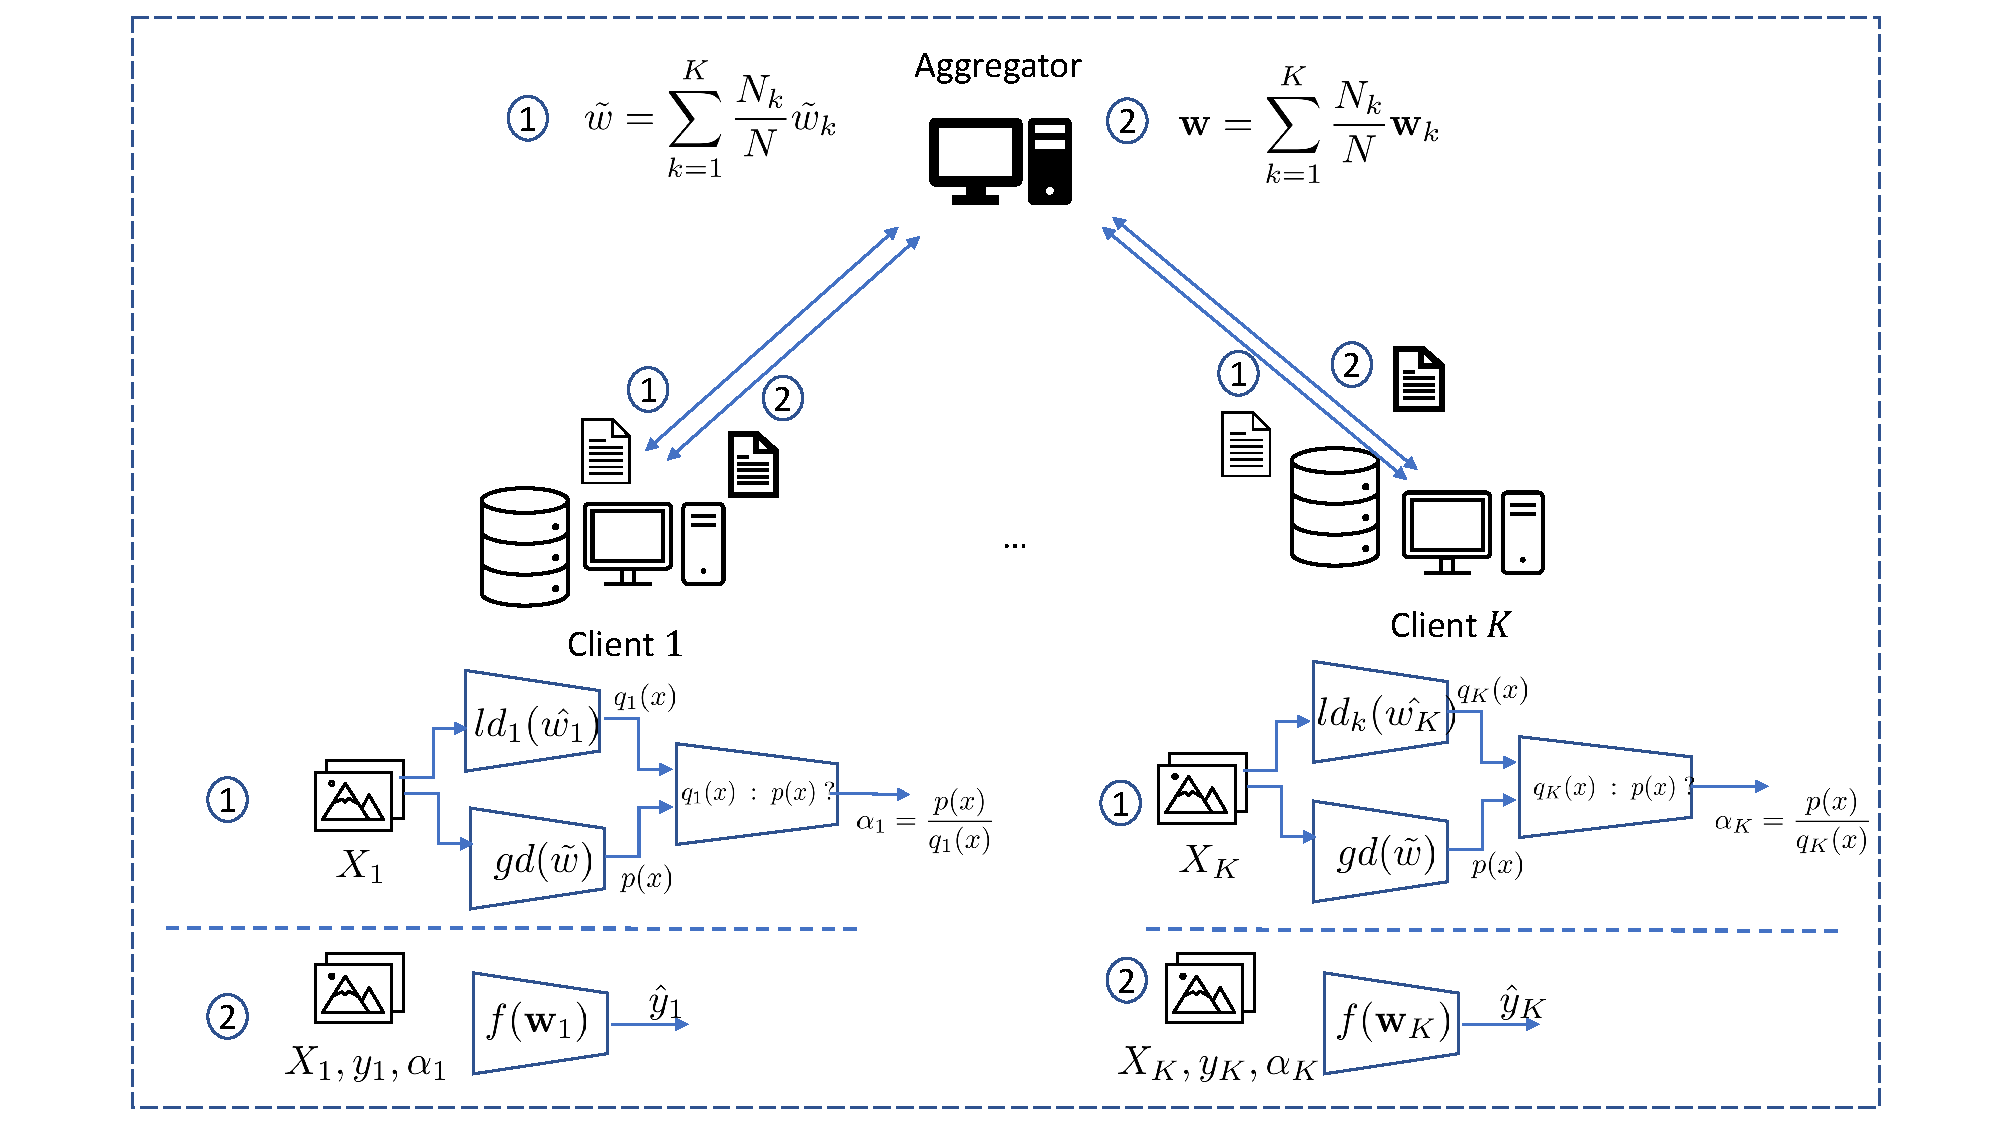
\includegraphics[width=0.85\textwidth, trim={1cm 0.1cm 1cm 0.3cm},clip]{Figures/FL}
		\caption{ \MethodnameShort{} Framework: The proposed framework has two phases. First, local and global probability density functions ($p(x),q(x)$) are estimated via MADE models leveraging FL procedures. Then, the sample weights $\alpha$ are computed by approximating density ratio via class probability estimation. Second, the machine learning tasks (e.g., classification) can be performed similar to a typical FL method (i.e., FedAvg) with the sample weights acquired from phase 1.} 
		\label{fig:framework} 

\end{figure*}  

\subsection{Sample Weights Design}
As we do not have sufficient information about the true distribution, we consider the combination of all clients' dataset distribution as our true distribution. Thus, we consider the probability density function (pdf) of the true distribution as 
\begin{equation}
\label{eq:sumdist}
	 p(\mathbf{x}) = \sum_{k=1}^{K}q_k(\mathbf{x}) ,
\end{equation}
where $q_k(\mathbf{x})$ represents the pdf of the $k^{th}$ client's data. 

To jointly learn a global model, the system finds the expectation of the loss function $l(g(\mathbf{x}),y)$ with sample $\x{}$ that drawn from the true distribution. The expected loss is formulated by the associated risk \cite{noauthor_empirical_2021} as follows:
\begin{align}
	\mathbb{E}[l(g(\mathbf{x}),y)] 
	% &= \iint l(g(\mathbf{\mathbf{x}}),y) p(\mathbf{x},y) d\mathbf{x}dy \label{eq:risk1}\\
	&= \iint l(g(\mathbf{x}),y) p(y|\mathbf{\mathbf{x}}) p(\mathbf{x}) d\mathbf{x}dy, \label{eq:risk} 
\end{align}
where $p(\mathbf{x},y)$ is the joint pdf of a sample $\mathbf{x}$ and its associated label $y$, and $p(y|\mathbf{x})$ is the conditional probability of a label $y$ given a sample $\mathbf{x}$. We also assume that for any client $k \in$ $\{1,...,K\}$ with local data distribution $q_k(\mathbf{x})$, the conditional probability of a label $y$ given a sample $\mathbf{x}$ is equivalent to that of the true distribution, namely
\begin{align}
	\label{eq:assumtion}
	 q_k(y|\mathbf{x}) = p(y|\mathbf{x}).
\end{align}

From Equation \ref{eq:sumdist}, \ref{eq:risk}, \ref{eq:assumtion}, and by multiplying with factor $\frac{q_k(\mathbf{x})}{q_k(\mathbf{x})}=1$, the expected loss in Equation \ref{eq:risk} can be expanded as follows:
\begin{align}
	\mathbb{E}[l(g(\mathbf{x}),y)]  &= \iint l(g(\mathbf{x}),y) p(y|\mathbf{x}) p(x) d\mathbf{x}dy,\\
	%&= \iint l(g(\mathbf{x}),y) p(y|\mathbf{x}) \frac{q_k(\mathbf{x})}{q_k(\mathbf{x})}  p(\mathbf{x}) d\mathbf{x}dy	 \\
	&= \iint l(g(\mathbf{x}),y) q_k(y|\mathbf{x}) \frac{q_k(\mathbf{x})}{q_k(\mathbf{x})}  p(\mathbf{x}) d\mathbf{x}dy \\
	&= \iint l(g(\mathbf{x}),y) q_k(\mathbf{x},y) \frac{p(\mathbf{x})}{q_k(\mathbf{x})}  d\mathbf{x}dy.    \label{eq:expectedloss}
\end{align}
The objective of the global model thus amounts to minimize the empirical risk over all $K$ clients' datasets:
\begin{equation}
	\begin{aligned}
	\underset{g}{\text{minimize}}
	 \sum_{k=1}^{K} \frac{1}{N_k}\sum_{j=1}^{N_k} \alpha_k^j \:l(g(\mathbf{x}_k^j),y_k^j)), \label{eq:optimation}
	\end{aligned}
\end{equation} 

where $\mathbf{x}_k^j$, $y_k^j$ are the $j^{th}$ sample and its label. $N_k$ is the number of samples in the $k^{th}$ client's dataset. $\alpha_k^j$ is the corresponding sample weight computed as
\begin{equation}
\begin{aligned}
	\boxed{\alpha_k^j = \frac{ \px{}{}}{q_k(\mathbf{x})}  = \frac{ \sum_{i=1}^{K}q_i(\mathbf{x}) }{q_k(\mathbf{x})}. }  
	\label{eq:alpha}.
\end{aligned}
\end{equation}

Our problem becomes minimizing the summation of the loss functions (Equation \ref{eq:optimation}) over all clients. For each client, the loss function is minimized over local samples with the corresponding $j^{th}$ sample weight of the client $k^{th}$, $\alpha_k^j$. The sample weights could be estimated by the density ratio between the true distribution (global distribution) and the client distributions (local distributions). For each client, the local distribution can be estimated using its local data. However, the challenge is to achieve the true distribution without having access to other clients' data. To solve this, we leverage a neural network-based density estimation model to learn the global density function via a typical federated learning procedure. Thus, clients can implicitly exchange some statistical information, while still preserving the privacy in client data.          

\subsection{Probability Density Approximation}
\label{sec:densityapproximation}
To estimate global density and preserve client privacy at the same time, we propose to leverage a neural network-based density estimation so that we can exchange local density information (via models' weights) with the aggregator without sharing the raw data. In this work, we leverage a well-known method, namely, Masked Autoencoder for Distribution Estimation (MADE, \cite{MADE}), which is briefly reviewed in Section \ref{sec:made}. Elaborately, each client aims to estimate its local probability density $q_k(\mathbf{x})$ using its own dataset, and all $K$ clients jointly estimate the global probability density $p(\mathbf{x}) = q_1(\mathbf{x})+...+q_K(\mathbf{x})$. Learned MADE models are used to approximate local probability density functions, and the global MADE model approximates the global probability density. The learning process is described as follows.    

The $k^{th}$ client learns a local density estimation model $ld_k(\hat{w}_k)$ (where $ld(\cdot)$ approximates density estimation function with parameter $\hat{w}$) using its local data. It then jointly learns a global density estimation model $gd(\tilde{w})$ (where $gd(\cdot)$ represents the global density function with the parameter $\tilde{w}$) using the procedure similarly to FedAvg \cite{OriginFL}. Specifically, for the local model density estimation models, each client train a MADE model on its local data until the loss function can not be improved. For the global density estimation model, each client trains its data locally for a certain number of iterations, and then model parameters are sent to an aggregator for the aggregation. Since clients might own different number of samples, a weight of ${N_k}/N$ (where $N_k$ and $N$ are the number of samples of the $k^{th}$ client and the the total number of samples over all clients) is used for adjusting client parameter significance, similar to FedAvg. After aggregating all clients' model parameters, the aggregator shares global model parameters to all clients. The steps are repeated until the validation loss starts increasing. The global MADE model aggregation from $K$ clients at iteration $t$ can be described as follows:
\begin{equation}
\begin{aligned}
 \tilde{w}^t = \frac{N_k}{N}\sum_{k=1}^{K} \tilde{w}^t_k 
\end{aligned}
\end{equation}

\subsection{Sample Weight Approximation}
\label{sec:weightapproximation}
After the local and global density approximations by MADE models are fully learned ( Section \ref{sec:densityapproximation}), we can estimate sample weights in Equation \ref{eq:alpha}. Since MADE models output vectors of conditional probabilities for each element in the d-dimensional input $\mathbf{x}$, an intuitive way to compute $p(\mathbf{x})$ is to multiply all the conditional probabilities. However, as $\px{}{}$ vanishes when any of the conditional probabilities vanishes, we instead keep the output as a vector of conditional probabilities (same size as input) and approximate the density ratio in Equation \ref{eq:alpha} using a class probability estimation method inspired by \cite{densityratio}. The method aims at training a binary classifier to output a probability that represents the ratio between $\px{}{}$ and $\qx{}{}$. The solution detail is described in the rest of this subsection. 

After each client receives the final global MADE model and trains its own local MADE, it starts to evaluate sample weights for its local data. The training data of the $k^{th}$ client, $X_k$, is then fed into both the global MADE (the global MADE is downloaded to clients so that this step can be done locally) and the local MADE to estimate $\px{}{}$ and $\qx{k}{}$, respectively. Denote $\ubold{}$ as the output vector of density estimation models, and $l$ be the pseudo label indicating whether it is sampled from the global destination ($l=1$) or the local distribution ($l=0$). Each client then trains a binary classifier to differentiate whether the output $\ubold$ comes from $\px{}{}$ or $\qx{k}{}$. Outputs of the two MADE models (the sample size of each output is $N_k$) are concatenated to a new vector dataset including samples $\{(\ubold{}_k^i,l_k^i) \}_{i=1}^{2N_k}$, and is used to train the binary classifier. The conditional probabilities of the binary classification model $h(\ubold,w_h)$ (where $\ubold$ is the input variable , $w_h$ is the model parameter) can be approximated as following: 
\begin{align}
	\Prob(\ubold | l=0 )  \propto  \qx{k}{}  ,\;\;\;\;
    \Prob(\ubold | l=1 )  \propto \px{}{}.
\end{align}

From Bayes' rule, we have
\begin{align}
	\frac{\px{}{}}{\qx{}{}} &= \frac{\Prob(\ubold | l=1 )}{ \Prob(\ubold | l=0 ) }       
	= \left( \frac{\Prob(l=1| \ubold ) \Prob(\ubold)}{\Prob(l=1)} \right)     
	\left( \frac{\Prob(l=0)} {\Prob(l=0| \ubold ) \Prob(\ubold)}\right)  \label{eq:pq1}\\
	 &= \frac{  \Prob(l=1|\ubold )  \Prob(l=0) }{ \Prob(l=0|\ubold )  \Prob(l=1)  }.  \label{eq:pq2} 
\end{align}

We approximate the marginal probability ratio between two distributions ( $\Prob(l=0)$  and $\Prob(l=1)$) by the number of samples from the two distributions $N_k$ over the concatenated dataset size ($2N_k$).Thus,  We have
 	$\frac{ \Prob(l=0) }{ \Prob(l=1)  } = \frac{N_k}{2N_k} \frac{2N_k}{N_k}=1. \label{eq:marginalratio}$

The density ratio then can be estimated as follows:
\begin{align}
\frac{\px{}{}}{\qx{}{}} &= \frac{  \Prob(l=1|\ubold )  }{ \Prob(l=0|\ubold )   } 
	= \frac{  \Prob(l=1|\ubold )  }{ 1 - \Prob(l=1|\ubold )   }. \label{eq:ratio2}
\end{align}, 
where $\Prob(l=1|\ubold{})$ is the classifier's probability-liked output indicating how likely an input vector $\ubold$ comes from the global probability $\px{}{}$. 
 
To summarize, the $j^{th}$ training sample of client $k$, $\x_k^j$, is fed into the client's local MADE model to achieve its corresponding density estimation $\ubold{}_k^j$. $\ubold{}_k^j$ is then fed into the binary classification function $h(\ubold)$ to achieve the class probability $ \Prob(l=1|\ubold_k^j ) $. This is used to estimate the sample weight $\alpha_k^j$ (Equation \ref{eq:alpha}) based on Equation \ref{eq:ratio2}. In words, the binary classification model $h(\ubold,w_h)$ is expected to return higher weights for samples that are likely belonging to the true distribution and vise versa. 

\subsection{Learning With Skewed Distribution Data Across clients }
After acquiring sample weights, each client starts to train the model on the local dataset and corresponding sample weights for a machine learning task (e.g., classification) as a typical FL framework. In this work, we follow the procedure introduced by FedAvg to learn the global model. The aggregator aggregates clients' local models as follows:
\begin{equation}
\begin{aligned}
\mathbf{w}^t = \frac{N_k}{N}\sum_{k=1}^{K} \mathbf{w}^t_k 
\end{aligned}
\end{equation}
where $\mathbf{w}^t$ and $\mathbf{w}^t_k$ are the global and local model parameter of $k^{th}$ client at the $t^{th}$ iteration.

\section{Privacy leakage analysis}
\label{sec:privacyAnalysis}
In this section, we discuss the privacy leakage of our method compared to the conventional FL. Similar to many other works, we utilize additional information to alleviate the negative impact of non-IID data, i.e., parameters of MADE models. However, these parameters might contain distribution information of clients’ data. However, we prove that the more clients are involved in the FL training process, the less information is leaked. The detail is described as follows. 
    
Assume each client samples their own data point ${\hat Z}_k \sim Q_k$ independently, and let  $\Theta$ be a random variable taking values in $\llbracket 1,K \rrbracket$ with $\prob[\Theta = k] = \kappa_k$ and independent of ${\hat Z}_k$ for each $k \in \llbracket 1,K \rrbracket$. Note that ${\hat Z}_\Theta \sim P$, and one may quantify the privacy leakage of client $k$'s data through the knowledge of $P$ by the mutual  information between ${\hat Z}_k$ and ${\hat Z}_\Theta$, as given by
\begin{equation}
\begin{aligned}
I({\hat Z}_k;{\hat Z}_\Theta) & \leq I({\hat Z}_k;{\hat Z}_\Theta, \Theta)
   =  I({\hat Z}_k; \Theta) + I({\hat Z}_k;{\hat Z}_\Theta | \Theta)
   \\ &= I({\hat Z}_k;{\hat Z}_\Theta | \Theta) = \sum_{i=1}^K \prob[\Theta = i] I({\hat Z}_k;{\hat Z}_i) = \kappa_k H({\hat Z}_k).
\end{aligned}
\end{equation}
%
In other words, the privacy leakage is proportional to $\kappa_k$, which decreases to $0$ as long as $\kappa_k = O(1/K)$ and $K \rightarrow \infty$.

\section{Experiments}
\label{sec:experiments}
In this section, we conduct several experiments to evaluate the proposed method on non-IID FL scenarios with three real image datasets (MNIST, Chest-Xray and FEMNIST). Our FL system goal is to learn a global classifier leveraging data from all clients. The classification accuracy is used as a metric to evaluate the performance of the proposed method. The communication cost is evaluated by counting the number of iterations needed for clients to exchange model parameters with the aggregator. We compare our method with other state-of-the-art methods, e.i., FedAvg, FedProx, FedBN, and FedROD. 

\subsection{Datasets \& non-IID setting.}
In this Section, we describe how datasets are used in our experiments. We categorize our dataset into two groups, simulated non-IID dataset (MNIST) and real non-IID datasets (Femnist \& Chest Xray). The first one contains images that have already been combined together so that our partitioning process is considered for sampling from the same contribution. Thus, we added different levels of noise to each client to simulate the feature skewness as inspired by settings in \cite{abs-2102-02079}, and \cite{FedProto}. The second group's data are collected from different sources so that they are considered to be non-IID by nature. All the data are normalized and clipped to the range of [0,1] before training. Each client's data is split to 85\% and 15\% for training and testing sets, respectively. The detail of the datasets is described as follows.  

\subsubsection{Simulated non-IID: MNIST}
MNIST dataset \cite{deng2012mnist} contains 60,000 (1x28x28) gray scale images of 10 digits (0-9). The number of unique output labels is 10 representing 10 digits. To mimic feature skewness, we split data equally into \parties{} partitions and add different level of noise to each client's data as inspried by the skewness simulation in \cite{abs-2102-02079}. The noise is drawn from Gaussian distribution with a mean of 0 and different values of standard deviations. More specifically, the $k^{th}$ client $(k \in [0,99])$ is added noise with the variance of $k*x/100$ where $x$ is the added noise variance.  

\subsubsection{Real non-IID: Femnist \& Chest Xray}
FEMNIST dataset is downloaded from https://leaf.cmu.edu/, which is considered a benchmark dataset for real non-IID data. It contains handwritten images of 62 digits and characters (corresponding to 62 unique labels) from different writers and strokes. In this study, we randomly select \parties{} different writers (each of them owns more than 300 images to avoid overfitting) and assign their data to \parties{} clients. The average sample size of clients is 387.47, and the standard deviation is 83.04. All images are resized to a (32x32) grayscale and normalized to the range of [0,1] before inputting to models.

The Chest-Xray dataset, which contains pneumonia and normal chest xray images, are collected from different sources (i.e., COVID-19 \cite{covid19}, Shenzhen Hospital \cite{Shenzhen}, and University of California San Diego (UCSD) \cite{Kermany2018LabeledOC}) with different image sizes, colors and potentially taken from different medical devices. Thus, we consider this dataset non-IID by nature. After partitioning the data into \parties{} clients, the mean and standard deviation of the client sample size are 325.50 and 63.74, respectively. All images are converted to grayscale and resized to (32x32). There are two unique output labels (binary classification) to predict chest xray images are normal or abnormal.

\subsection{Implementation Detail}
\subsubsection{Baselines}
We compare our methods with different methods, i.e., FedAvg, FedProx, FedBN, and FedROD. While most implementation details are taken from the initial parameter sets in original papers, we also tune suggested parameters and report the results that give the best values. For FedROD, the results are reported for the hyper-parameter $\mu$ of 1. We also tried other values in the set {1, 5, 10, 20} and found that the results are very similar. For FedProx, we tuned the parameter $\mu$ with the candidates of {0.001, 0.01, 0.1, 1} and reported the value of 0.01, 1, 0.01 for the three datasets, Chest-Xray, FEMNIST, MNIST, respectively. 

\subsubsection{Federated Learning Classification Model} We use shallow Convolutional Neural Networks (CNN) for the classification of image datasets. The models are constructed by two 5x5 convolutional layers (32 and 32 channels for Chest-Xray, 128 and 128 channels for FEMNIST, 32 and 32 channels for MNIST). Each convolutional layer is followed by 2x2 max pooling and batch normalization layers. A fully connected layer with 16 neurons is added on the top of the models. The input and output sizes are designed to fit each dataset scenario (i.e., image size and the number of unique labels). We use stochastic gradient descent (SGD) with a learning rate of 0.01 for the optimizers. Local iterations are set to 2 for all datasets. Global iterations are set to 1500 for FEMNIST and MNIST, and 500 for Chest-Xray. 

\subsubsection{Density Estimation Model (MADE)} Density estimation models (MADE) are constructed by neural networks and the hyper-parameters are taken directly from the initial setting for MNIST dataset by the original work \cite{MADE}. More detail, the models include a 500-neuron hidden layer. We also tried different settings of MADE. For example, the number of layers was tuned within the set of {1,2,3} and 500 neurons in each layer. However, the three settings gave very similar results. Thus, we select one hidden layer as it is the optimized setting. The model's input and output sizes are the flattened size of images. For example, the input and output size is 784 for MNIST dataset with an image size of 28x28. The maximum iteration is 500, and the training process is stopped when the validation loss starts increasing. Other hyper-parameters are taken directly from \cite{MADE}.

\subsubsection{Sample Weight Approximation} In order to compute the sample weight $alpha$, we use a shallow, fully connected neural network to discriminate the density estimation output vectors coming from which of the two distribution density functions $\px{}{}$ or $\qx{}{}$. The model contains a 100-neuron hidden layer with Relu activation function. The output layer contains one neuron with Sigmoid activation function. All models applied a learning rate of 0.01, and SGD optimization were used in the training process. The training process is terminated if the loss function is not significantly reduced.

\subsection{Results}
\begin{figure*}[ht!]
	\centering
	%[trim=left bottom right top, clip]
	\begin{subfigure}[t]{0.3\linewidth}	
		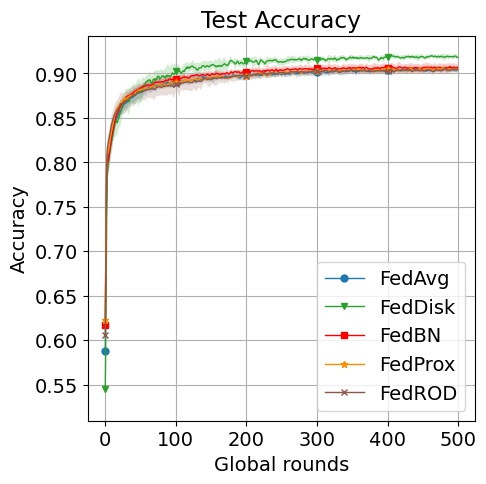
\includegraphics[width=\linewidth]{Figures/xray/test_acc}
		\caption{Chest-Xray }
		\label{fig:acc_xray}
	\end{subfigure}
	\hspace{0.01em}%
	\begin{subfigure}[t]{0.3\linewidth}
		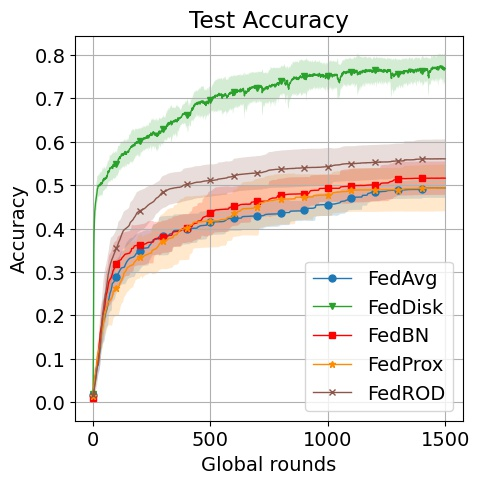
\includegraphics[width=\linewidth]{Figures/femnist/test_acc}
		\caption{FEMNIST}
		\label{fig:acc_femnist}
	\end{subfigure}
	\hspace{0.01em}%
	\begin{subfigure}[t]{0.3\linewidth}	
		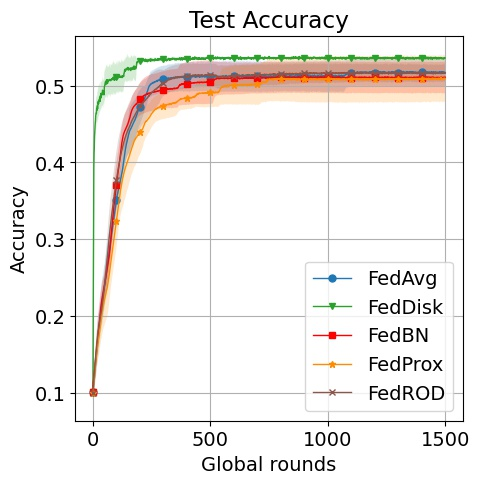
\includegraphics[width=\linewidth]{Figures/mnist/test_acc}
		\caption{MNIST (NoiseVar 0.3)  }
		\label{fig:acc_mnist}
	\end{subfigure}
	\caption{Global model's average test accuracy during aggregation process. For MNIST dataset, clients' data were added noise with the mean of zero and variance of 0.3  }
	\label{fig:acc_all}
\end{figure*}

\begin{figure*}[ht!]
	\centering
	%[trim=left bottom right top, clip]
	\begin{subfigure}[t]{0.3\linewidth}	
		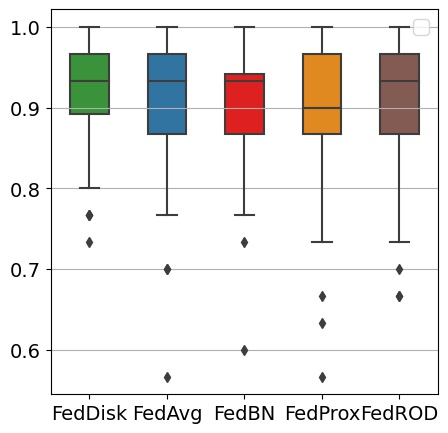
\includegraphics[width=\linewidth]{Figures/xray/ClientAcc}
		\caption{Chest-Xray }
		\label{fig:cl_acc_xray}
	\end{subfigure}
	\hspace{0.01em}%
	\begin{subfigure}[t]{0.3\linewidth}
		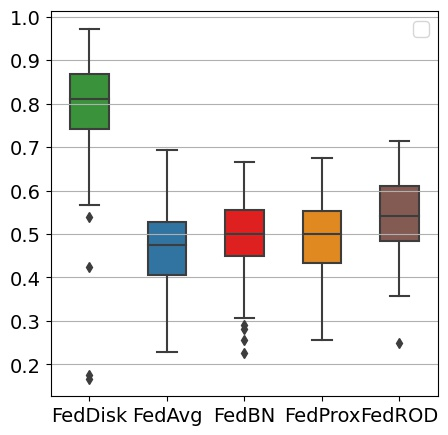
\includegraphics[width=\linewidth]{Figures/femnist/ClientAcc}
		\caption{FEMNIST}
		\label{fig:cl_acc_femnist}
	\end{subfigure}
	\hspace{0.01em}%
	\begin{subfigure}[t]{0.3\linewidth}	
		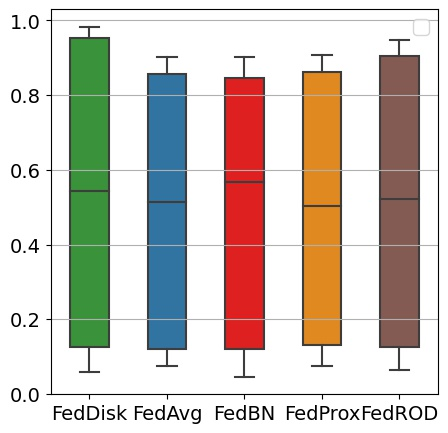
\includegraphics[width=\linewidth]{Figures/mnist/ClientAcc}
		\caption{MNIST (NoiseVar 0.3) }
		\label{fig:cl_acc_mnist}
	\end{subfigure}
	\caption{Test accuracy percentiles, min, max and median plot of \parties{} clients for different datasets and methods. }
	\label{fig:cl_acc_all}
\end{figure*}

\subsubsection{Classification Accuracy} Figure \ref{fig:acc_all} shows the average of the \parties{} clients' testing accuracies over training iterations. The shaded regions illustrate the standard deviation over five trials. Overall, \MethodnameShort{} significantly outperforms other methods in terms of classification accuracy. For example, in Figure \ref{fig:acc_xray} for Chest-Xray dataset, \MethodnameShort{} with an accuracy of 92\% outperforms others with the highest accuracy of 90.5\%. For FEMNIST dataset (Figure \ref{fig:acc_femnist}), our method achieved an accuracy of 78\% while others only reached the maximum accuracy of 56\% (FedROD). For MNIST, \MethodnameShort{} reached the accuracy of 54.5\% while others only obtained the highest accuracy of 51.7\%. 

Figure \ref{fig:cl_acc_all} shows the descriptive statistical accuracy results of \parties{} clients on different datasets. The colored rectangles contain 50\% of client accuracies. The colored rectangular's lower and upper edges show the middle values in the first and second half of the sorted clients' accuracies (lower quartile and higher quartile). The middle dash is the median value. The upper and lower dashes represent the min and max clients' accuracies. Dots illustrate outliers. Overall, the bars for \MethodnameShort{} are higher than others, meaning that most clients archive higher accuracy. Dots are also higher (Figure \ref{fig:cl_acc_xray} and \ref{fig:cl_acc_femnist}) for \MethodnameShort{}, showing that outlier clients are also improved. Especially, the bar for FEMNIST is significantly raised for \MethodnameShort{}, indicating that the proposed method significantly improved for this dataset. It is clear that the proposed method outperforms compared methods in all experimental datasets, including real-world non-IID and simulated non-IID settings.

\subsubsection{Performance over different feature skewness levels}
\begin{figure*}[ht!]
	\centering
	%[trim=left bottom right top, clip]
	\begin{subfigure}[t]{0.3\linewidth}	
		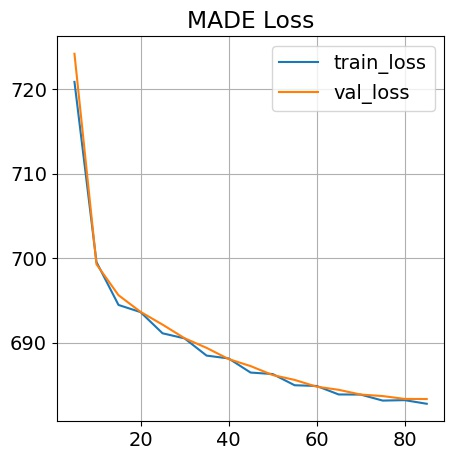
\includegraphics[width=\linewidth]{Figures/xray/MADE_loss}
		\caption{Chest-Xray }
		\label{fig:made_loss_xray}
	\end{subfigure}
	\hspace{0.01em}%
	\begin{subfigure}[t]{0.3\linewidth}
		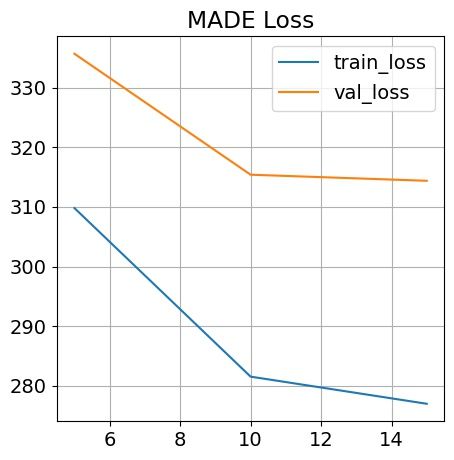
\includegraphics[width=\linewidth]{Figures/femnist/MADE_loss}
		\caption{FEMNIST}
		\label{fig:made_loss_femnist}
	\end{subfigure}
	\hspace{0.01em}%
	\begin{subfigure}[t]{0.3\linewidth}	
		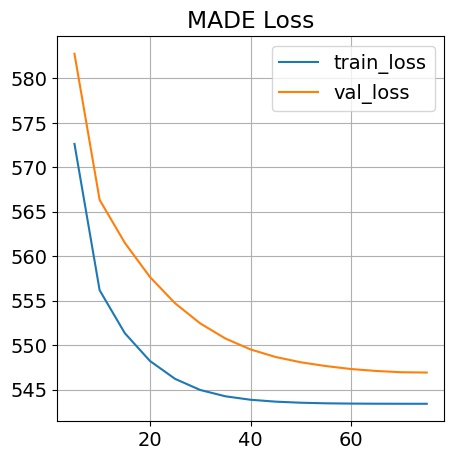
\includegraphics[width=\linewidth]{Figures/mnist/MADE_loss}
		\caption{MNIST (NoiseVar 0.3)  }
		\label{fig:made_loss_mnist}
	\end{subfigure}
	\caption{Average validation and train losses during training the global MADE models. The training processes were stopped if the validation loss starts increasing. }
	\label{fig:made_loss}
\end{figure*}
We also evaluate the proposed method over different skewness levels by conducting experiments on MNIST dataset with varying values of added noise variance. Figure \ref{fig:accvsnoise} shows the average accuracy for FedDisk and FedAvg on MNIST dataset over added noise variance values. It illustrates that the proposed method is more resilient to different skewness levels as the gap between accuracy results of the two approaches becomes more significant when the added noise variance increases. When the added noise variance is as low as 0.1, both methods closely achieve an accuracy of 94\%. However, when the added noise is as high as 0.7, the gap between \MethodnameShort{} and FedAvg accuracies becomes more significant as the accuracy is 45\% for \MethodnameShort{} and 25\% for FedAvg. Overall, the experiment shows that the proposed method is more resilient to the skewness level than the conventional method FedAvg.
\begin{figure}[ht!]
	\centering
	%[trim=left bottom right top, clip]
	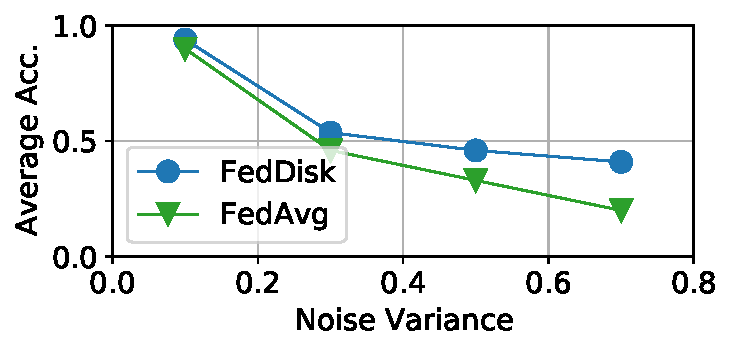
\includegraphics[width=0.8\linewidth]{Figures/Accuracy_vs_noise}
	\caption{FedDisk and FedAvg accuracy on different added noise variance.}	
	\label{fig:accvsnoise}
\end{figure}

\subsubsection{Communication Cost}
To evaluate the communication cost, we calculate the number of ``Effective Communication Rounds" (ECR). For \MethodnameShort{}, ECR include the communication rounds for exchanging MADE models and classification models. Figure \ref{fig:made_loss} show the aggregated training loss and validation loss for the global MADE model over communication rounds. The global MADE exchanging process stops when the validation loss starts increasing. For example, the proposed method needs 15 rounds for exchanging global MADE models in the case of FEMNIST dataset. The ECR for \MethodnameShort{} in the classification phase are calculated with the number of iterations that the proposed method needed to achieve the highest value of other methods gained. For example, for the FEMNIST dataset experiment shown in Figure \ref{fig:cl_acc_femnist}, \MethodnameShort{} only needs 105 rounds to reach the accuracy of 57\% (FedROD's accuracy), which is the highest accuracy among other experimental methods. Plus 15 rounds to exchange MADE model, \MethodnameShort{} only needs a total of 120 rounds to effectively reach the top comparison method accuracy. The ECRs of other methods are calculated with the number of exchanging classification model rounds until they reach their highest accuracy values.  
\begin{figure}[ht!]
	\centering
	%[trim=left bottom right top, clip]
	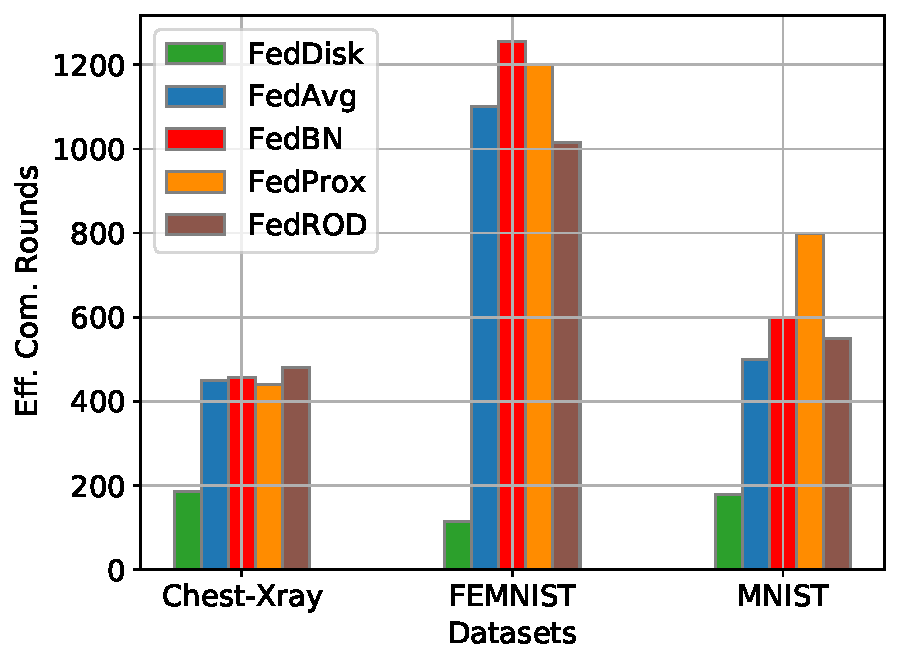
\includegraphics[width=0.85\linewidth]{Figures/Com.Rounds}
	\caption{Summary of ``Effective Communication Rounds" over 3 datasets. The Figure shows that \MethodnameShort{} is much more efficient in terms of communication cost.}	
	\label{fig:communication_round}
\end{figure}


Figure \ref{fig:communication_round} shows the summary of ``Effective Communication Rounds" for the three experimental datasets. As shown in the Figure, \MethodnameShort{} is the most effective method as it needs a lot fewer communication rounds to reach the highest accuracy among other methods. This is because the proposed method only needs a few number communication rounds for the global MADE model to be converged, and such statistical information accelerates the global classification model to reach high accuracy much faster compared to others. For example, for FEMNIST dataset, the \MethodnameShort{}'s ECR is only 120 (15 for MADE model exchange plus 105 for classification model exchange ), whereas others take more than 1000 iterations (a communication cost reduction of more than eight times). The communication cost reduction trend is also applied to other experimental datasets, Chest-Xray (2 times) and MNIST (2.5 times). Therefore, the proposed method not only improves the accuracy but also dramatically reduces the communication cost for the experimental datasets, which is one of the most critical concerns in Federated Learning.

      
\section{Conclusion}
\label{sec:conclusion}
In this work, we have proposed a FL method to tackle the issue of distribution skewed data. The technique utilizes a FL framework and a neural network-based density estimation model to derive training sample weights. This helps to adjust the global distribution without revealing clients' raw data. We also provide a privacy analysis for the extra information used in \MethodnameShort{} (i.e., the parameters of MADE models) and prove that the leakage information becomes less important when the number of clients increases. The experimental results show that the proposed method not only improves the FL accuracy but also significantly reduces communication costs. 

\balance


\bibliographystyle{plainnat}
\bibliography{egbib}

\end{document}



































